\section{Tareas de SocialNLP}


\section{Redes Neuronales}

\subsection{Brevísima historia}
\subsection{Definición}
\subsection{Multi-layer perceptron}
\subsection{Redes neuronales recurrentes}
\subsection{Optimización}


\section{Técnicas de representación de NLP}
\subsection{Word-embeddings}

\subsubsection{Sub-word embeddings}

\subsection{Modelos pre-entrenados}

\subsubsection{Transfer Learning}

\subsection{ELMo}
\begin{figure}
    \centering
    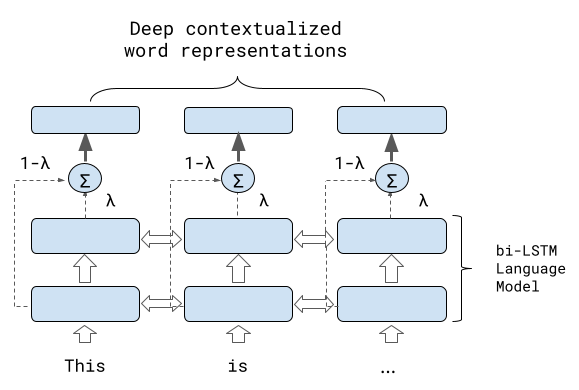
\includegraphics[width=0.65\textwidth]{img/ELMo.png}
    \caption{Ilustración de ELMo. Las dos capas inferiores representan un modelo de lenguaje bidireccional, y la superior representa una combinación lineal convexa de las salidas de las capas recurrentes}
    \label{fig:modelos_offenseval_hateval}
\end{figure}
\subsection{ULM-Fit}
\subsection{BERT}